

\documentclass{article}
\usepackage{hyperref}
\usepackage{graphicx}
\usepackage[utf8x]{inputenc}
\usepackage[T1,T2A]{fontenc}
\usepackage[russian,english]{babel}

\usepackage{amsmath,amssymb,amsthm,amsfonts}



\newtheorem{Def}{Definition}[section]
\newtheorem{theorem}{Theorem}
\newtheorem{statement}{Statement}
\newtheorem{Cnj}[Def]{Conjecture}
\newtheorem{Prop}[Def]{Property}
\newtheorem{example}{Example}[section]

\newcommand{\Li}{\mathrm{Li}}
\newcommand{\dx}{\mathrm{dx}~}
\newcommand{\dy}{\mathrm{dy}~}
\newcommand{\dz}{\mathrm{dz}}

\begin{document}
\title{Finite-size scaling of free energy in the dimer model on a hexagonal domain}

\author{A.A.~Nazarov$^{1}$\\
{\small
  $^{1}$Department of Physics, St. Petersburg State University,} \\
{\small  Ulyanovskaya 1, 198504 St.~Petersburg, Russia}\\
\small{email:antonnaz@gmail.com}
}
\date{}
\maketitle

\begin{abstract}
  We consider dimer model on a hexagonal lattice. This model can be seen as a ``pile of cubes in the
  corner''. The energy of configuration is given by the volume of the pile and the partition
  function is computed by the classical MacMahon formula or, more formally, by the determinant of
  Kasteleyn matrix. We use the expression for the partition function to derive the scaling behavior
  of free energy in the limit of lattice mesh tending to zero and temperature tending to infinity.
  We discuss the universality and physical meaning of expansion coefficients.
\end{abstract}


\section*{Introduction}
\label{sec:introduction}
The dimer model appeared in attempt to extend a statistical theory of perfect solutions in chemistry
to the case of liquid mixtures with molecules of two very distinct sizes \cite{Fowler-1937}. The
molecules were represented by the rigid tiles on a lattice and the number of tilings was
approximately estimated. But an exact computation was not accessible at the time.

In 1961, Kasteleyn \cite{P.W-1961}, Temperley and Fisher \cite{doi:10.1080/14786436108243366}
represented the partition function of the dimer model as a Pfaffian of the signed adjacency matrix
(``Kasteleyn matrix'') thus allowing the computation of the number of tilings and of free energy scaling limit.
This result was very elegantly used by Fisher to solve Ising model \cite{fisher1966dimer} and by Fan
and Wu \cite{Fan-1970} to compute free energy for a certain case of eight-vertex model.

Further studies of dimer models revealed the connection to the theory of alternating matrices
\cite{elkies1992alternating1,elkies1992alternating2}. Later, the well-known limit shape
phenomenon~\cite{vershik1977kerov} was discovered for dimer models. First, the ``Arctic circle''
theorem was proven for domino tilings of the domain in the form of ``Aztec diamond''
~\cite{1998math......1068J}. Then similar result was obtained for a hexagonal domain on the
hexagonal lattice~\cite{cohn1998shape}. Soon the connection of these results with the theory of
random matrices was established~\cite{johansson2002non}. The papers
\cite{kenyon2006dimers,kenyon2009lectures} present a detailed exposition of the limit shape
phenomenon in the dimer models.

Dimer models are the integrable lattice models of statistical physics that are now under an active
theoretical~\cite{zj2000,ferrari} and numerical investigation~\cite{ks2018}. Computation of
correlation functions is a common problem for all vertex models \cite{colomo2012approach} as well as
for dimer models. Another problem of great interest is the study of limit shapes in various cases
\cite{borodin2010q,di2018tangent}.

Configurations of dimer model on a hexagonal lattice are in one-to-one correspondence with the
configurations of five-vertex model that appears for certain choice of parameters in the well-known
six-vertex model \cite{kapitonov2012weighted,kapitonov2008five}.

Study of dimer models on various lattices and domains led to interesting connections with the
geometry of curved manifolds and with spectra of discrete and continuous Dirac and Laplace operators
\cite{kenyon2002laplacian,kenyon2000asymptotic}. Scaling limit of dimer model is proven to be
described by a Gaussian free-field theory \cite{kenyon2001dominos}, but finite-size corrections were
not considered previously. These corrections are important to close the gap between numerical
simulations and theoretical results.

We consider a particular case of the dimer model on a hexagonal domain of hexagonal lattice, that
can be seen as a ``pile of cubes in the corner''. The energy of configuration is the total number of
cubes. For this particular case we use an exact combinatorial formula for the partition function to
derive the expressions for scaling limit of free energy and first three terms of the finite-size
corrections. We show that the first term is identically zero. The second term is geometry-dependent
and is written explicitly in terms of elementary functions. The third term which encapsulates
logarithmic dependence on the mesh size is connected with the central charge of the effective field
theory.

This result is supported by numeric simulations presented in our previous publication
\cite{1742-6596-1135-1-012024}.

\section{Model definition}
\label{sec:model-definition}
The configurations of the dimer model are perfect matchings (sets of non-touching edges, covering
all the vertices) on some graph ${\cal G}$ with some choice of weights $\omega(e)$ on the edges. The
model is solvable on the bipartite graphs, i.e. the partition function can be computed if the
weights are introduced in such a way that for each face bounded by 0 mod 4 edges there is an odd
number of negative edge weights and each face with 2 mod 4 edges has an even number of of negative
edge weights. Then the signs of the edge weights form a so-called ``Kasteleyn orientation''on graph,
the weighting is called ``Kasteleyn weighting'' \cite{kenyon2001dominos,kenyon2009lectures}.

For a bipartite graph ${\cal G}$, color the vertices black and white in such a way that all the
vertices adjacent to the black one are white. Denote by $B, W$ the sets of black and white
vertices and by $b,w$ the elements of these sets. 

The weights can be encoded as the ``Kasteleyn matrix'' -- weighted, signed adjacency matrix ${\cal K}$ with
the matrix elements ${\cal K}(w,b)$ equal to the weight of the edge $w\to b$: ${\cal K}(w,b)=\omega(w\to b)$.

Then the partition function is equal to the absolute value of the determinant of the Kasteleyn
matrix\cite{P.W-1961,doi:10.1080/14786436108243366}: 
\begin{equation}
  \label{eq:15}
  Z=\sum_{\mathrm{conf}}\prod_{e\in \mathrm{conf}}w(e)=|\det {\cal K}|
\end{equation}

Kasteleyn matrix defines a discrete Dirac operator $D$, the action of $D$ on a function $f$ defined
on vertices is given by:
\begin{equation}
  \label{eq:16}
  (Df)(v)=\sum_{u}{\cal K}(v,u) f(u)
\end{equation}

Kenyon \cite{kenyon2002laplacian,kenyon2000asymptotic} and others \cite{sridhar2015asymptotic}
considered asymptotics of the determinants of the discrete Dirac and Laplace operators, the problem
that, as can be seen from the above, is very close to the scaling of the free energy. But the finite
size corrections to the free energy scaling were not computed. 
  
We consider coverings of the hexagonal domain on the hexagonal lattice consisting of the subsets of
lattice edges such that every vertex is the endpoint of exactly one edge.

We can draw a rhombus on a dual lattice around each edge in the configuration. The picture of
``cubes in the corner'' presented in the Fig.~\ref{dhf} is obtained. Let us write on the top of each
uppermost cube the height of its column of cubes. Looking at this picture from the top, we obtain a
height function defined on the rectangular domain of the square lattice. 

\begin{figure}[htbp]
\center{\scalebox{0.4}{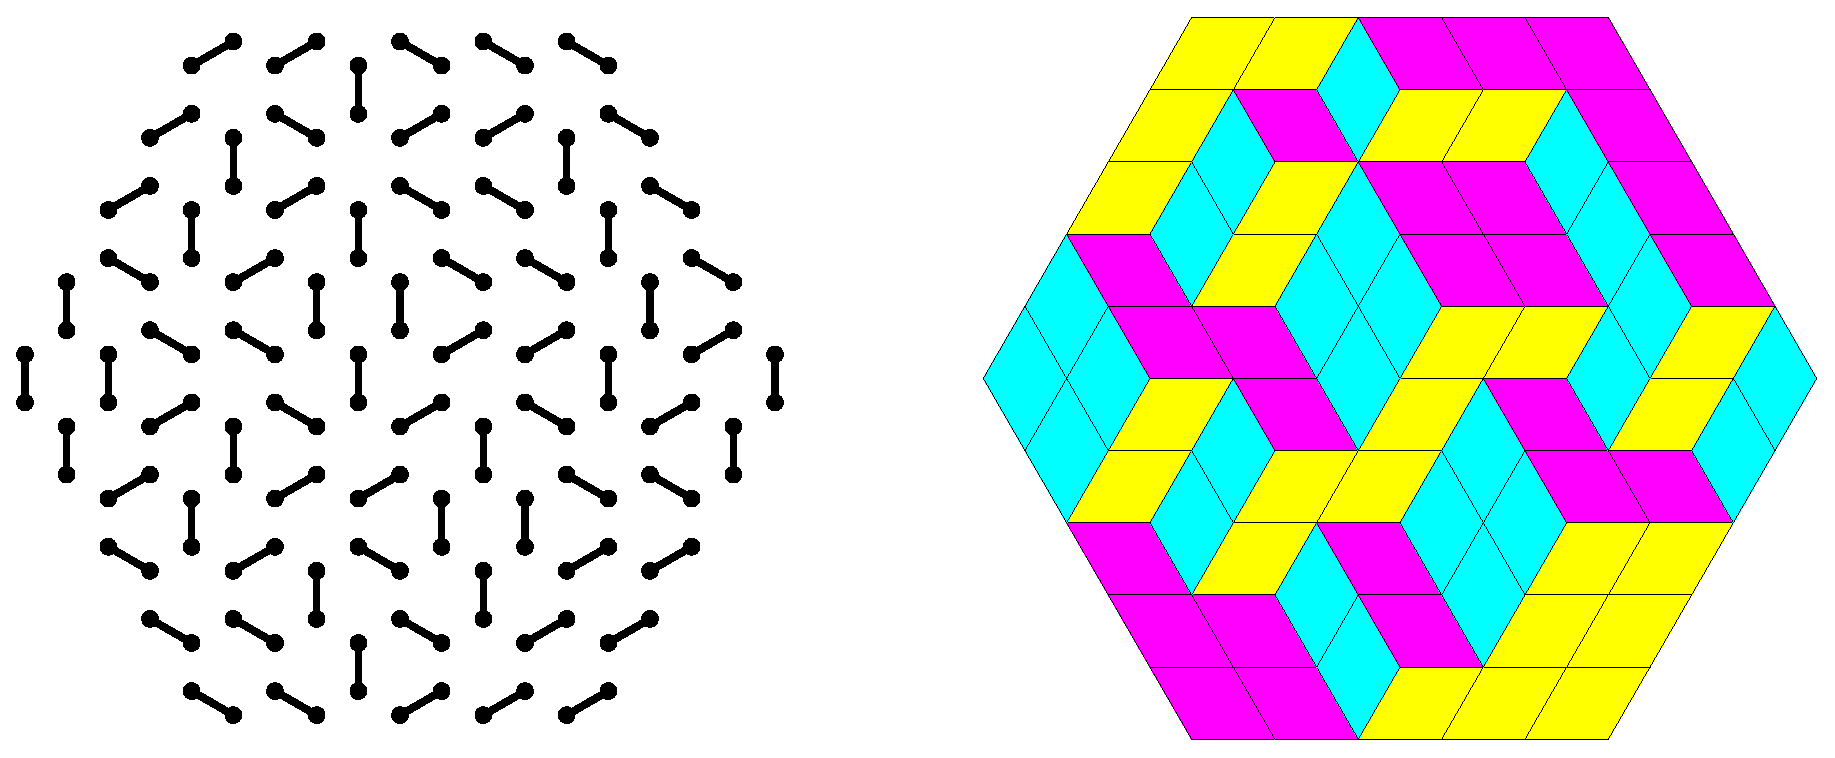
\includegraphics{loz.eps}}}
\caption{\label{dhf}A configuration of dimers on the hexagonal lattice and a corresponding picture
  of ``cubes in the corner''.}
\end{figure}

Let us define the sizes $M$, $N$, and $K$ of the sides of the hexagon.
The above description can be formalized by
%set of configurations of the model can be defined all possible ways to write
setting the non-negative numbers up to $K$ in the boxes of the rectangular $M\times N$ table so that a value in
each box is not greater than values in the adjacent upper and left boxes
\begin{equation}
  \label{eq:1}
  h_{ij}\leq h_{i-1,j},\quad h_{ij}\leq h_{i,j-1}.
\end{equation}

The weight of a particular configuration is given by the exponent of the volume of all cubes or by a
sum of the height function values:
\begin{equation*}
  \label{eq:10}
  E[conf]=\sum_{i,j} h_{ij}=\mathrm{Volume}
\end{equation*}
We set Boltzman constant equal to 1 and choose system of units in such a way that there is no
coupling constant in the expression for energy. Then the partition function is
\begin{equation*}
  \label{eq:14}
  Z=\sum_{conf} e^{-\frac{E[conf]}{T}}=\sum_{conf}q^{\mathrm{Volume}[conf]}, 
\end{equation*}
where $q=\exp\left(-1/T\right)$ .

For this particular case, the partition function is given by the classical Macmahon combinatorial
formula~\cite{vuletic2009generalization}
\begin{equation}
  \label{eq:12}
   Z[M,N,K,q]=\prod_{i=1}^{M}\prod_{j=1}^{N}\prod_{k=1}^{K}\frac{1-q^{i+j+k-1}}{1-q^{i+j+k-2}}
\end{equation}


MacMahon formula is obtained for the following definition of the Kasteleyn matrix. Embed the
hexagonal lattice in the complex plane $\mathbb{C}$ in such a way that some edges are parallel to
the real line with and corresponding vertices have coordinates with integer real and imaginary
parts. Then take
\begin{eqnarray}
  \label{eq:18}
  {\cal K}(w,b)=q^{\Re w+\Im w} \quad \mathrm{if}\quad \Im w=\Im b\\
  {\cal K}(w,b)=1 \quad \mathrm{if}\quad \Im w\neq\Im b
\end{eqnarray}


The   free energy per site is defined as$^{*}$
\footnote{For convenience we omit the factor $\frac{1}{T}$ in the usual definition of the free energy.}
\begin{equation*}
  \label{eq:17}
  % \frac{f}{T}
  f=-\frac{1}{V}\ln Z(M,N,K,q)
\end{equation*}
Here $V$ is the number of vertices, it is twice the number of dimers and twice the number of  cube faces:
\begin{equation*}
  \label{eq:19}
  V=2(MN+NK+MK)
\end{equation*}

We are interested in the scaling limit, combined with the thermodynamic limit, when $ T\to \infty,$
and $M,N,K\to \infty$, such that ratios $\frac{M}{T}=a,\quad \frac{N}{T}=b, \quad \frac{K}{T}=c$
remain fixed. In what follows we use $\varepsilon=\frac{1}{T}$, which can be seen as the scale of
the model, e.g. mesh size due to our choice of the system of units.

In the next section we compute the asymptotic expansion of the free energy $f$ in $\varepsilon$ and
derive $\varepsilon$-independent closed expressions for the first several coefficients in this
expansion.
  
\section{The computation of the free energy asymptotic expansion}
\label{sec:free-energy-scaling}
First we substitute MacMahon formula \eqref{eq:12} into the free energy definition \eqref{eq:17} and
obtain
\begin{equation}
  \label{eq:20}
    %-\frac{f}{T}
    f=-\frac{1}{V}\ln Z =- \sum_{i=1}^{M} \sum_{j=1}^{N} \sum_{k=1}^{K} \frac{1}{V}
  \ln\left(\frac{1-e^{-\varepsilon (i+j+k)} e^{\varepsilon}}{1-e^{-\varepsilon (i+j+k)} e^{2\varepsilon}}\right)
\end{equation}
Expanding the exponents $e^{\varepsilon}, e^{2\varepsilon}$ and logarithms in powers of $\varepsilon$ we obtain


\begin{multline}
  \label{eq:4}
  %\frac{f}{T}
  f=- \sum_{i=1}^{M} \sum_{j=1}^{N} \sum_{k=1}^{K} \frac{1}{V}\left\{
    \varepsilon g(i\varepsilon,j\varepsilon,k\varepsilon)+
    \frac{3}{2}\varepsilon^{2}\left[g(i\varepsilon,j\varepsilon,k\varepsilon)+g(i\varepsilon,j\varepsilon,k\varepsilon)^{2}\right]\right.\\
  \left.+\frac{7}{6}\varepsilon^{3}\left[g(i\varepsilon,j\varepsilon,k\varepsilon)+3 g(i\varepsilon,j\varepsilon,k\varepsilon)^{2}+
      2 g(i\varepsilon,j\varepsilon,k\varepsilon)^{3}\right]\right\}  + \mathcal{O}(\varepsilon^{4})
\end{multline}
%% Wrong power of $\varepsilon$ below!!

Here and below we will use the notation:
\begin{equation}
  \label{eq:5}
  g(x,y,z)=\frac{1}{e^{x+y+z}-1}
\end{equation}

This expression looks like a combination of Riemann sums for some integrals. Note that these sums
are finite, but some of the corresponding integrals are divergent.


Let $G$ be an analytic function in the cube $[0,a]\times[0,b]\times[0,c]$, then
\begin{multline}
  \label{eq:21}
  \int_{0}^{a} \int_{0}^{b}\int_{0}^{c}G(x,y,z) \dx\; \dy\;
  \dz\approx\sum_{i=1}^{M}\sum_{j=1}^{N}\sum_{k=1}^{K}\left\{\varepsilon^{3}G\left(i\varepsilon,j\varepsilon,k\varepsilon\right)-\right.\\
  \left.-\left[\frac{\varepsilon^{4}}{2}\left((\partial_{x}+\partial_{y}+\partial_{z})G\right)(i\varepsilon,j\varepsilon,k\varepsilon)\right]+\right.\\
  \left.\varepsilon^{5}\left(\frac{1}{6}(\partial_{x}^{2}+\partial_{y}^{2}+\partial_{z}^{2})+\frac{1}{4}(\partial_{x}\partial_{y}+\partial_{x}\partial_{z}+\partial_{y}\partial_{z})\right)G\left(i\varepsilon,j\varepsilon,k\varepsilon\right)
  \right\}+\mathcal{O}(\varepsilon^{6})
\end{multline}
This formula can be easily derived by dividing the volume of integration into cubes with side
$\varepsilon$ and substituting Taylor series for $G$ into integrals.

We can use this formula to approximate sums by integrals. Similar formula can be written for a
function of two variables and double sums. We will not need higher order terms, but will use the
approximation:
\begin{equation}
\label{eq:8}
  \sum_{j=1}^{N}\sum_{k=1}^{K}\varepsilon^{2}G\left(i\varepsilon,j\varepsilon,k\varepsilon\right)\approx \int_{0}^{b}\int_{0}^{c}G(i\varepsilon,y,z) \dy\; \dz+\mathcal{O}(\varepsilon^{3}))
\end{equation}



Note that
\begin{equation}
  \label{eq:6}
  \begin{array}{c}
    \partial_{x}g(x,y,z)=-g(x,y,z)-g(x,y,z)^{2}\\
    \partial_{x}^{2}g(x,y,z)=g(x,y,z)+3g(x,y,z)^{2}+2g(x,y,z)^{3}
  \end{array}
\end{equation}

Taking this into account and using the relation \eqref{eq:21} to express the triple sum
$ \sum_{i=1}^{M} \sum_{j=1}^{N} \sum_{k=1}^{K} \frac{1}{V}    \varepsilon g(i\varepsilon,j\varepsilon,k\varepsilon)$
in \eqref{eq:4} as the integral plus corrections, we obtain
\begin{multline}
\label{eq:23}
 f=-\frac{1}{2(ab+bc+ca)}\left\{\int_{0}^{a} \int_{0}^{b}\int_{0}^{c}\frac{\dx \dy \dz}{e^{x+y+z}-1}+\right.\\
  \left.+\sum_{i=1}^{M}\sum_{j=1}^{N}\sum_{k=1}^{K}\frac{\varepsilon^{5}}{12}\left[g(i\varepsilon,j\varepsilon,k\varepsilon)+3
      g(i\varepsilon,j\varepsilon,k\varepsilon)^{2}+2
      g(i\varepsilon,j\varepsilon,k\varepsilon)^{3}\right]\right\}
\end{multline}
Due to the equations \eqref{eq:6}, the corrections are of the same form as the higher order terms in
$\varepsilon$. The linear in $\varepsilon$ term in \eqref{eq:4} is cancelled by three partial
derivatives in \eqref{eq:21}. The coefficient of the quadratic term is changed by the addition of
second derivatives from \eqref{eq:21} to $\frac{1}{12}$.


There is no singularity in the sum, but
$\int_{0}^{a} \int_{0}^{b}\int_{0}^{c}\frac{\dx \dy \dz}{(\exp(x+y+z)-1)^{3}}$ diverges
logarithmically. So we can not just apply the integral representation~\eqref{eq:21} directly.

We apply the formula \eqref{eq:8} to the internal sums in the triple sum, since there is no
singularity in $\frac{1}{\left((\exp(i\varepsilon+j\varepsilon+k\varepsilon)-1\right)^{3}}$ for
$i\neq 0$:

\begin{equation}
  \label{eq:9}
\sum_{i=1}^{M}\left(\sum_{j=1}^{N}\sum_{k=1}^{K}\frac{\varepsilon^{5}}{12}
      \frac{e^{2(i\varepsilon+j\varepsilon+k\varepsilon)}+e^{i\varepsilon+j\varepsilon+k\varepsilon}}{\left(e^{i\varepsilon+j\varepsilon+k\varepsilon}-1\right)^{3}}  \right)\approx
    \frac{\varepsilon^{3}}{12}\sum_{i=1}^{M} \int_{0}^{b}\int_{0}^{c}
      \left(\frac{e^{2(i\varepsilon+y+z)}+e^{i\varepsilon+y+z}}{\left(e^{i\varepsilon+y+z}-1\right)^{3}}\right) \dy \dz+\mathcal{O}(\varepsilon^{3})
\end{equation}

The double integral can be taken explicitly, so we obtain
\begin{equation}
  \label{eq:11}
  \frac{\varepsilon^{3}}{12}\sum_{i=1}^{M}\left(     \frac{1}{e^{b+c+i\varepsilon}-1}+
  \frac{1}{1-e^{b+i\varepsilon}}+\frac{1}{1-e^{c+i\varepsilon}}+\frac{1}{e^{i\varepsilon}-1}\right)
\end{equation}

The function $\frac{1}{e^{x}-1}$ has a divergence, so we can not apply integral approximation directly. We first need to 
subtract and add $\frac{1}{i\varepsilon}$. The sum over $i$ of this term can be approximated using Euler formula:
\begin{equation}
    \label{eq:24}
    \sum_{i=1}^{M}\frac{1}{i}=\frac{1}{M}\sum_{i=1}^{M}\frac{1}{i/M}=\int_{\frac{1}{M}}^{1}\frac{\dx}{x}+\gamma+O(\varepsilon)=-\ln\varepsilon+\ln a+\gamma+O(\varepsilon)
  \end{equation}
Thus we get the integral %%!!!!!
\begin{multline}
  \label{eq:13}
    \frac{\varepsilon^{3}}{12}\left[\sum_{i=1}^{M}\left(     \frac{1}{e^{b+c+i\varepsilon}-1}+
      \frac{1}{1-e^{b+i\varepsilon}}+\frac{1}{1-e^{c+i\varepsilon}}+\frac{1}{e^{i\varepsilon}-1}-\frac{1}{i\varepsilon}\right)-\ln\varepsilon+\ln a+\gamma+\mathcal{O}(\varepsilon^{3})\right]\approx\\
   \frac{\varepsilon^{2}}{12}\left[\int_{0}^{a}\left(     \frac{1}{e^{b+c+x}-1}+
      \frac{1}{1-e^{b+x}}+\frac{1}{1-e^{c+x}}+\frac{1}{e^{x}-1}-\frac{1}{x}\right)\dx-\ln\varepsilon+\ln a+\gamma\right]+\mathcal{O}(\varepsilon^{3})    
\end{multline}
The integral is now taken explicitly, it is equal to
\begin{multline}
  \label{eq:22}
     \frac{\varepsilon^{2}}{12}\left[\int_{0}^{a}\left(     \frac{1}{e^{b+c+x}-1}+
         \frac{1}{1-e^{b+x}}+\frac{1}{1-e^{c+x}}+\frac{1}{e^{x}-1}-\frac{1}{x}\right)\dx-\ln\varepsilon+\ln a+\gamma\right]=\\
     \frac{\varepsilon^{2}}{12}\left[\ln \left(\frac{(e^{a}-1)(e^{b}-1)(e^{c}-1)(e^{a+b+c}-1)}{a (e^{a+b}-1)(e^{b+c}-1)(e^{a+c}-1)}\right)-\ln\varepsilon+\ln a+\gamma\right]
\end{multline}

  

The term $\ln a$ is cancelled by the  and symmetry between $a,b,c$ is restored.
Substituting this approximation into the expression \eqref{eq:23} we obtain 
 the final expression:
\begin{multline}
  \label{eq:3}
 f=-\frac{1}{2(ab+bc+ca)}\left\{\int_{0}^{a} \int_{0}^{b}\int_{0}^{c}\frac{\dx \dy \dz}{e^{x+y+z}-1}+\right.\\
  \left.+\frac{\varepsilon^{2}}{12}\left[\ln\left(\frac{(e^{a}-1)(e^{b}-1)(e^{c}-1)(e^{a+b+c}-1)}{(e^{a+b}-1)(e^{b+c}-1)(e^{a+c}-1)}\right)-
      \gamma\right]+\frac{\varepsilon^{2}}{12}\ln \varepsilon\right\} +\mathcal{O}(\varepsilon^{3})
\end{multline}

\section{Physical meaning of the expansion coefficients}
\label{sec:accur-expans-phys}

The expansion  (\ref{eq:3}) can be written as
\begin{equation}
  \label{eq:26}
  f=f_{0}+f_{1}\varepsilon +f_{2}\varepsilon^{2}\ln\varepsilon+ f_{3}\varepsilon^{2},
\end{equation}
where the coefficients are
\begin{equation}
  \label{eq:27}
  f_{0}=-\frac{1}{2(ab+bc+ca)}\int_{0}^{a} \int_{0}^{b}\int_{0}^{c}\frac{\dx \dy \dz}{e^{x+y+z}-1},
\end{equation}
\begin{equation}
  \label{eq:28}
  f_{1}=0,
\end{equation}
\begin{equation}
  \label{eq:30}
  f_{2}=-\frac{1}{2(ab+bc+ca)}\frac{1}{12},
\end{equation}
and
\begin{equation}
  \label{eq:29}
  f_{3}=-\frac{1}{2(ab+bc+ca)}\frac{1}{12}\left[\ln\left(\frac{(e^{a}-1)(e^{b}-1)(e^{c}-1)(e^{a+b+c}-1)}{(e^{a+b}-1)(e^{b+c}-1)(e^{a+c}-1)}\right)-
    \gamma\right].
\end{equation}

In the paper \cite{1742-6596-1135-1-012024} we have presented results of Monte Carlo simulations using
Metropolis and Wang-Landau algorithms that support the form of expansion (\ref{eq:26}). In
particular we got $f_{1}=0.04\pm 0.04$ which is consistent with $f_{1}=0$. 

In the scaling limit $\varepsilon\to 0$ so called ``limit shape phenomenon''~\cite{1998math......1068J,cohn1998shape}
appears in the dimer model. The areas around the corners of the domain are ``frozen'' with height
function values being fixed. An analytical ``Arctic curve'' delimits frozen regions from the region
where the behavior is described by the effective free field theory
\cite{kenyon2009lectures,kenyon2008height,kenyon2006dimers}.

The behavior (\ref{eq:26}) of the logarithm of the partition function is generic in two-dimensional
models \cite{cardy1988finite}.

First two terms $f_{0}$ and $f_{1}$ are interpreted as a bulk and
boundary free energies in the corresponding field theory. Since we have $f_{1}=0$, we can conclude
that boundary tension is zero.
The value of the first term $f_{0}$ can be rewritten using polylogarithm functions as
\begin{multline}
  \label{eq:34}
  f_{0}=\frac{1}{2(ab+bc+ca)}\left[abc + \Li_{3}(e^{a})+\Li_{3}(e^{b})+\Li_{3}(e^{c})-
    \Li_{3}(e^{a+b})\right.\\
  \left.-\Li_{3}(e^{b+c})-    \Li_{3}(e^{a+c})+    \Li_{3}(e^{a+b+c})-\zeta(3)\right]
\end{multline}
Here Riemann zeta function appears as a particular value of polylogarithm $\Li_{3}(1)=\zeta(3)$. 

The term proportional to the logarithm of the scale $\varepsilon$ is also universal
\cite{cardy1988finite} and should appear in all two-dimensional theories with boundary. In the paper
\cite{cardy1988finite} it was argued that on a manifold of a characteristic length $L$ with a smooth
boundary such a term must have the following form:
\begin{equation}
  \label{eq:31}
  \delta F = -\frac{1}{6}{\bf c} \chi \ln L,
\end{equation}
where ${\bf c}$ is central charge of the effective field theory and $\chi$ is the Euler characteristic of
the manifold
\begin{equation}
  \label{eq:32}
  \chi=2-2 h-b,
\end{equation}
where $h$ is the number of handles and $b$ is the number of boundaries. 

Since the non-frozen domain is delimited by a smooth boundary, we have $\chi=1$ and we interpret
$2(ab+bc+ca)$ as a volume of the domain, thus
\begin{equation}
  \label{eq:33}
  \delta F = \left(2(ab+bc+ca)\right) f_{2}\ln\varepsilon,
\end{equation}
which together with formula \eqref{eq:30} suggests the value of central charge
${\bf c}=\frac{1}{2}$. This value is in agreement with the identification of the dimer model with
free fermions in the paper \cite{dijkgraaf2009dimer}.

The last term $f_{3}$ depends only on the shape of the domain through $a,b,c$ with a universal
contribution that is equal to the Euler constant $\gamma$. We conjecture that Euler constant will
appear even for a different choice of Kasteleyn weighting, due to the treatment of logarithmic
divergency. In the future work we will consider coordinate dependent values of $q$ and more complex
geometries, as was done in the paper \cite{okounkov2007random}, to check this suggestion. 


\section*{Conclusion and outlook}
\label{sec:conclusion}

In the present paper we computed the asymptotic expansion of the free energy in the dimer model on a
hexagonal domain of the hexagonal lattice. We've discussed the physical meaning of the expansion
coefficients and argued that our results support the identification of the scaling behavior of the
dimer model with the free-fermion field theory.

In further work we will show the connection of the expansion coefficients with the spectral
properties of Dirac operator on the non-frozen domain and study the universality of the presented
expressions by considering the model on more generic domain geometries with the non-uniform
Kasteleyn weighting with $q$ depending on the coordinate.

\section*{Acknowledgments}
\label{sec:acknowledgements}
I am grateful to professor Nikolai Reshetikhin for his guidance in this work. I thank Pavel Belov
for useful discussions and general support.

I thank the organizers and participants of the conference MQFT-2018 for the opportunity
to present our results and useful discussions.

This research is supported by RFBR grant No. 18-01-00916.

\bibliographystyle{utphys}
\bibliography{listing,bibliography,dimers}{} 
\end{document}
